\documentclass[1p]{elsarticle_modified}
%\bibliographystyle{elsarticle-num}

%\usepackage[colorlinks]{hyperref}
%\usepackage{abbrmath_seonhwa} %\Abb, \Ascr, \Acal ,\Abf, \Afrak
\usepackage{amsfonts}
\usepackage{amssymb}
\usepackage{amsmath}
\usepackage{amsthm}
\usepackage{scalefnt}
\usepackage{amsbsy}
\usepackage{kotex}
\usepackage{caption}
\usepackage{subfig}
\usepackage{color}
\usepackage{graphicx}
\usepackage{xcolor} %% white, black, red, green, blue, cyan, magenta, yellow
\usepackage{float}
\usepackage{setspace}
\usepackage{hyperref}

\usepackage{tikz}
\usetikzlibrary{arrows}

\usepackage{multirow}
\usepackage{array} % fixed length table
\usepackage{hhline}

%%%%%%%%%%%%%%%%%%%%%
\makeatletter
\renewcommand*\env@matrix[1][\arraystretch]{%
	\edef\arraystretch{#1}%
	\hskip -\arraycolsep
	\let\@ifnextchar\new@ifnextchar
	\array{*\c@MaxMatrixCols c}}
\makeatother %https://tex.stackexchange.com/questions/14071/how-can-i-increase-the-line-spacing-in-a-matrix
%%%%%%%%%%%%%%%

\usepackage[normalem]{ulem}

\newcommand{\msout}[1]{\ifmmode\text{\sout{\ensuremath{#1}}}\else\sout{#1}\fi}
%SOURCE: \msout is \stkout macro in https://tex.stackexchange.com/questions/20609/strikeout-in-math-mode

\newcommand{\cancel}[1]{
	\ifmmode
	{\color{red}\msout{#1}}
	\else
	{\color{red}\sout{#1}}
	\fi
}

\newcommand{\add}[1]{
	{\color{blue}\uwave{#1}}
}

\newcommand{\replace}[2]{
	\ifmmode
	{\color{red}\msout{#1}}{\color{blue}\uwave{#2}}
	\else
	{\color{red}\sout{#1}}{\color{blue}\uwave{#2}}
	\fi
}

\newcommand{\Sol}{\mathcal{S}} %segment
\newcommand{\D}{D} %diagram
\newcommand{\A}{\mathcal{A}} %arc


%%%%%%%%%%%%%%%%%%%%%%%%%%%%%5 test

\def\sl{\operatorname{\textup{SL}}(2,\Cbb)}
\def\psl{\operatorname{\textup{PSL}}(2,\Cbb)}
\def\quan{\mkern 1mu \triangleright \mkern 1mu}

\theoremstyle{definition}
\newtheorem{thm}{Theorem}[section]
\newtheorem{prop}[thm]{Proposition}
\newtheorem{lem}[thm]{Lemma}
\newtheorem{ques}[thm]{Question}
\newtheorem{cor}[thm]{Corollary}
\newtheorem{defn}[thm]{Definition}
\newtheorem{exam}[thm]{Example}
\newtheorem{rmk}[thm]{Remark}
\newtheorem{alg}[thm]{Algorithm}

\newcommand{\I}{\sqrt{-1}}
\begin{document}

%\begin{frontmatter}
%
%\title{Boundary parabolic representations of knots up to 8 crossings}
%
%%% Group authors per affiliation:
%\author{Yunhi Cho} 
%\address{Department of Mathematics, University of Seoul, Seoul, Korea}
%\ead{yhcho@uos.ac.kr}
%
%
%\author{Seonhwa Kim} %\fnref{s_kim}}
%\address{Center for Geometry and Physics, Institute for Basic Science, Pohang, 37673, Korea}
%\ead{ryeona17@ibs.re.kr}
%
%\author{Hyuk Kim}
%\address{Department of Mathematical Sciences, Seoul National University, Seoul 08826, Korea}
%\ead{hyukkim@snu.ac.kr}
%
%\author{Seokbeom Yoon}
%\address{Department of Mathematical Sciences, Seoul National University, Seoul, 08826,  Korea}
%\ead{sbyoon15@snu.ac.kr}
%
%\begin{abstract}
%We find all boundary parabolic representation of knots up to 8 crossings.
%
%\end{abstract}
%\begin{keyword}
%    \MSC[2010] 57M25 
%\end{keyword}
%
%\end{frontmatter}

%\linenumbers
%\tableofcontents
%
\newcommand\colored[1]{\textcolor{white}{\rule[-0.35ex]{0.8em}{1.4ex}}\kern-0.8em\color{red} #1}%
%\newcommand\colored[1]{\textcolor{white}{ #1}\kern-2.17ex	\textcolor{white}{ #1}\kern-1.81ex	\textcolor{white}{ #1}\kern-2.15ex\color{red}#1	}

{\Large $\underline{11a_{276}~(K11a_{276})}$}

\setlength{\tabcolsep}{10pt}
\renewcommand{\arraystretch}{1.6}
\vspace{1cm}\begin{tabular}{m{100pt}>{\centering\arraybackslash}m{274pt}}
\multirow{5}{120pt}{
	\centering
	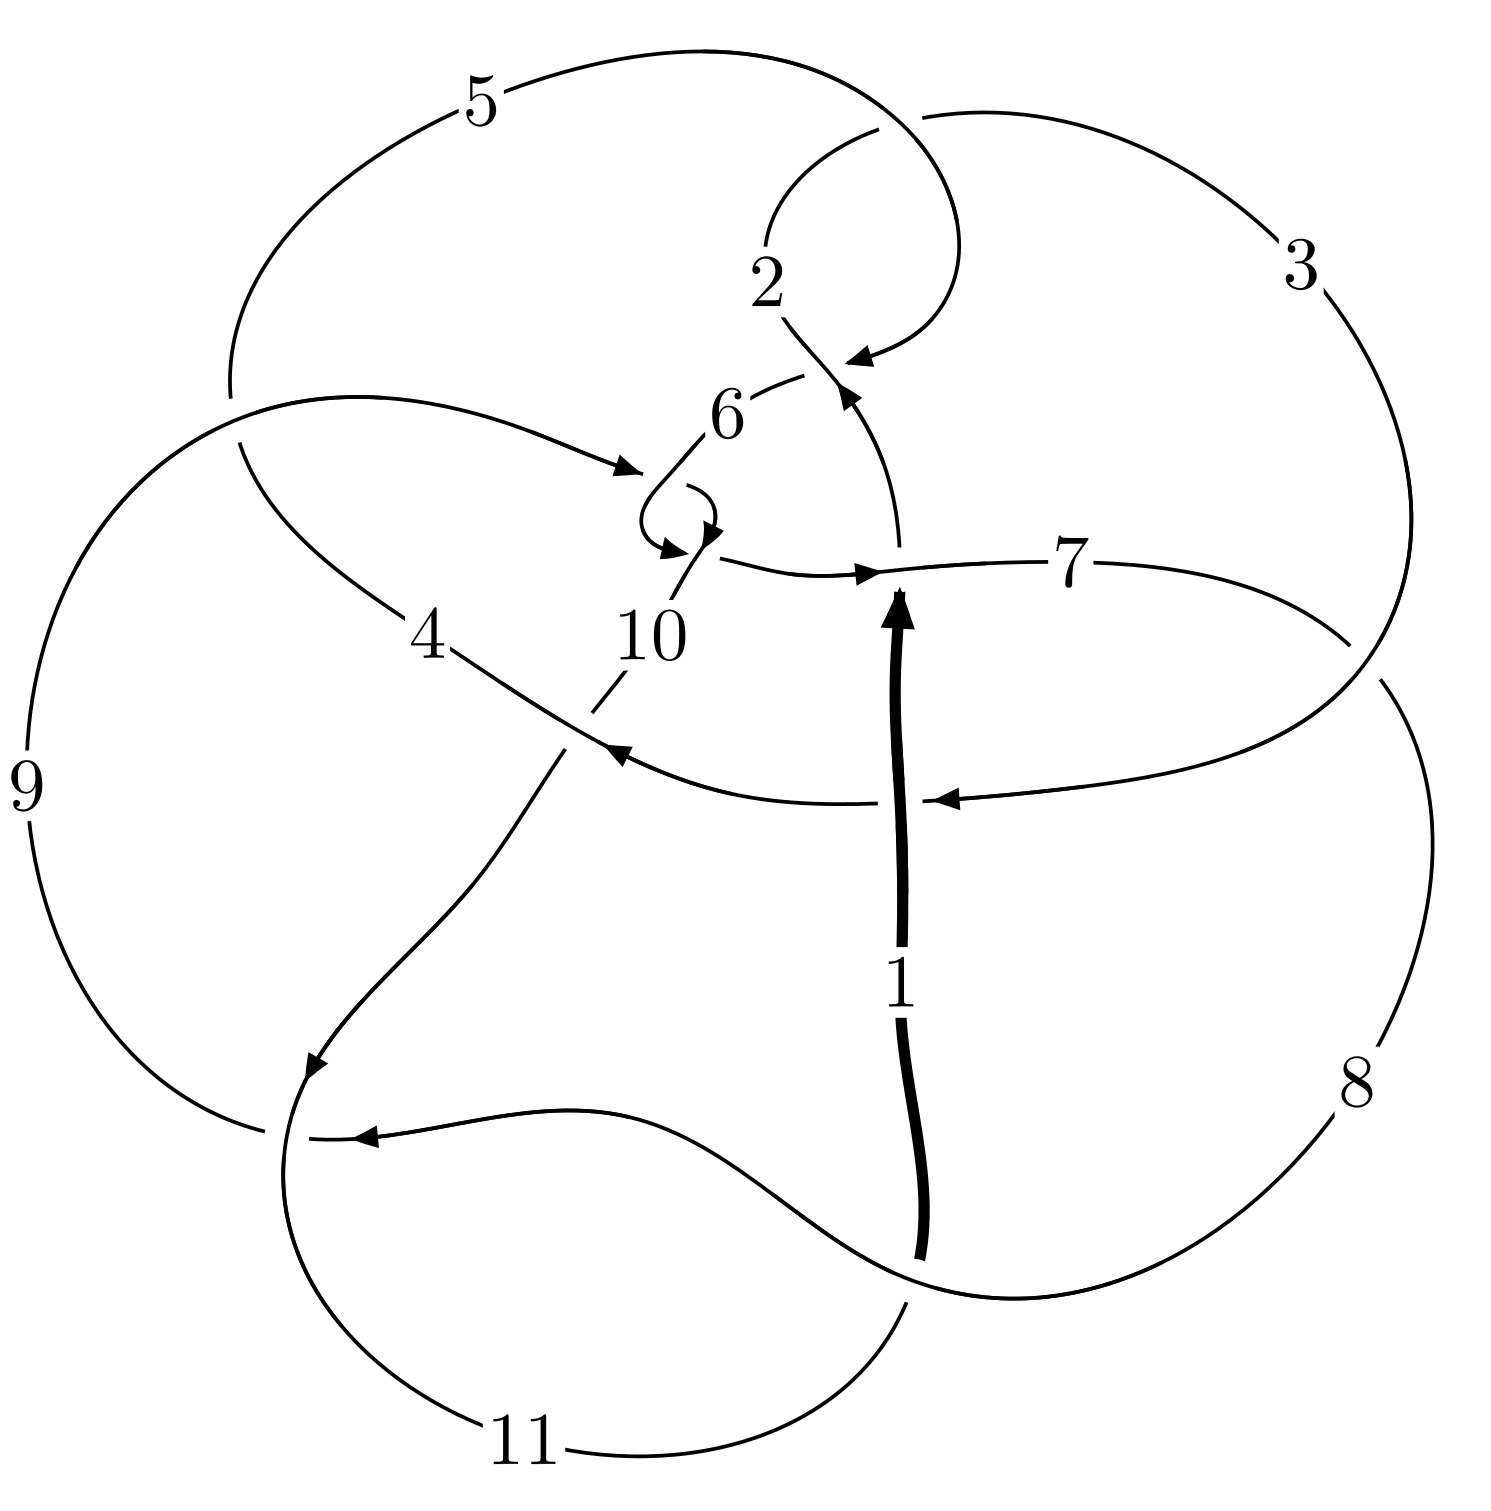
\includegraphics[width=112pt]{../../../GIT/diagram.site/Diagrams/png/525_11a_276.png}\\
\ \ \ A knot diagram\footnotemark}&
\allowdisplaybreaks
\textbf{Linearized knot diagam} \\
\cline{2-2}
 &
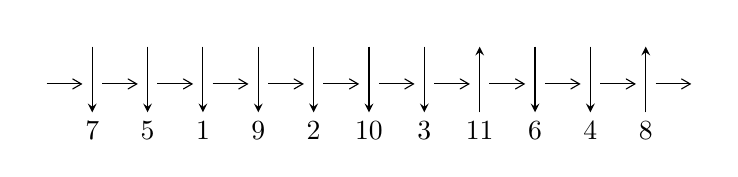
\begin{tikzpicture}[x=20pt, y=17pt]
	% nodes
	\node (C0) at (0, 0) {};
	\node (C1) at (1, 0) {};
	\node (C1U) at (1, +1) {};
	\node (C1D) at (1, -1) {7};

	\node (C2) at (2, 0) {};
	\node (C2U) at (2, +1) {};
	\node (C2D) at (2, -1) {5};

	\node (C3) at (3, 0) {};
	\node (C3U) at (3, +1) {};
	\node (C3D) at (3, -1) {1};

	\node (C4) at (4, 0) {};
	\node (C4U) at (4, +1) {};
	\node (C4D) at (4, -1) {9};

	\node (C5) at (5, 0) {};
	\node (C5U) at (5, +1) {};
	\node (C5D) at (5, -1) {2};

	\node (C6) at (6, 0) {};
	\node (C6U) at (6, +1) {};
	\node (C6D) at (6, -1) {10};

	\node (C7) at (7, 0) {};
	\node (C7U) at (7, +1) {};
	\node (C7D) at (7, -1) {3};

	\node (C8) at (8, 0) {};
	\node (C8U) at (8, +1) {};
	\node (C8D) at (8, -1) {11};

	\node (C9) at (9, 0) {};
	\node (C9U) at (9, +1) {};
	\node (C9D) at (9, -1) {6};

	\node (C10) at (10, 0) {};
	\node (C10U) at (10, +1) {};
	\node (C10D) at (10, -1) {4};

	\node (C11) at (11, 0) {};
	\node (C11U) at (11, +1) {};
	\node (C11D) at (11, -1) {8};
	\node (C12) at (12, 0) {};

	% arrows
	\draw[->,>={angle 60}]
	(C0) edge (C1) (C1) edge (C2) (C2) edge (C3) (C3) edge (C4) (C4) edge (C5) (C5) edge (C6) (C6) edge (C7) (C7) edge (C8) (C8) edge (C9) (C9) edge (C10) (C10) edge (C11) (C11) edge (C12) ;	\draw[->,>=stealth]
	(C1U) edge (C1D) (C2U) edge (C2D) (C3U) edge (C3D) (C4U) edge (C4D) (C5U) edge (C5D) (C6U) edge (C6D) (C7U) edge (C7D) (C8D) edge (C8U) (C9U) edge (C9D) (C10U) edge (C10D) (C11D) edge (C11U) ;
	\end{tikzpicture} \\
\hhline{~~} \\& 
\textbf{Solving Sequence} \\ \cline{2-2} 
 &
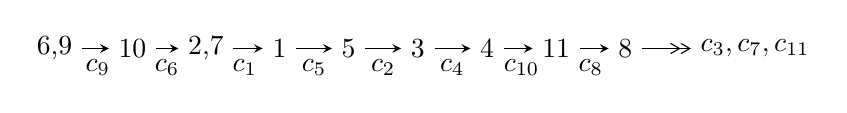
\begin{tikzpicture}[x=25pt, y=7pt]
	% node
	\node (A0) at (-1/8, 0) {6,9};
	\node (A1) at (1, 0) {10};
	\node (A2) at (33/16, 0) {2,7};
	\node (A3) at (25/8, 0) {1};
	\node (A4) at (33/8, 0) {5};
	\node (A5) at (41/8, 0) {3};
	\node (A6) at (49/8, 0) {4};
	\node (A7) at (57/8, 0) {11};
	\node (A8) at (65/8, 0) {8};
	\node (C1) at (1/2, -1) {$c_{9}$};
	\node (C2) at (3/2, -1) {$c_{6}$};
	\node (C3) at (21/8, -1) {$c_{1}$};
	\node (C4) at (29/8, -1) {$c_{5}$};
	\node (C5) at (37/8, -1) {$c_{2}$};
	\node (C6) at (45/8, -1) {$c_{4}$};
	\node (C7) at (53/8, -1) {$c_{10}$};
	\node (C8) at (61/8, -1) {$c_{8}$};
	\node (A9) at (10, 0) {$c_{3},c_{7},c_{11}$};

	% edge
	\draw[->,>=stealth]	
	(A0) edge (A1) (A1) edge (A2) (A2) edge (A3) (A3) edge (A4) (A4) edge (A5) (A5) edge (A6) (A6) edge (A7) (A7) edge (A8) ;
	\draw[->>,>={angle 60}]	
	(A8) edge (A9);
\end{tikzpicture} \\ 

\end{tabular} \\

\footnotetext{
The image of knot diagram is generated by the software ``\textbf{Draw programme}" developed by Andrew Bartholomew(\url{http://www.layer8.co.uk/maths/draw/index.htm\#Running-draw}), where we modified some parts for our purpose(\url{https://github.com/CATsTAILs/LinksPainter}).
}\phantom \\ \newline 
\centering \textbf{Ideals for irreducible components\footnotemark of $X_{\text{par}}$} 
 
\begin{align*}
I^u_{1}&=\langle 
-6.63399\times10^{307} u^{102}-1.76777\times10^{308} u^{101}+\cdots+4.99508\times10^{308} b-1.10340\times10^{310},\\
\phantom{I^u_{1}}&\phantom{= \langle  }-1.30225\times10^{312} u^{102}-4.26703\times10^{312} u^{101}+\cdots+9.25589\times10^{311} a-2.15727\times10^{314},\\
\phantom{I^u_{1}}&\phantom{= \langle  }u^{103}+4 u^{102}+\cdots+469 u+109\rangle \\
I^u_{2}&=\langle 
425805 u^{22}+807010 u^{21}+\cdots+75671 b-868327,\\
\phantom{I^u_{2}}&\phantom{= \langle  }637990 u^{22}+1114149 u^{21}+\cdots+75671 a-1825552,\;u^{23}+u^{22}+\cdots- u+1\rangle \\
\\
\end{align*}
\raggedright * 2 irreducible components of $\dim_{\mathbb{C}}=0$, with total 126 representations.\\
\footnotetext{All coefficients of polynomials are rational numbers. But the coefficients are sometimes approximated in decimal forms when there is not enough margin.}
\newpage
\renewcommand{\arraystretch}{1}
\centering \section*{I. $I^u_{1}= \langle -6.63\times10^{307} u^{102}-1.77\times10^{308} u^{101}+\cdots+5.00\times10^{308} b-1.10\times10^{310},\;-1.30\times10^{312} u^{102}-4.27\times10^{312} u^{101}+\cdots+9.26\times10^{311} a-2.16\times10^{314},\;u^{103}+4 u^{102}+\cdots+469 u+109 \rangle$}
\flushleft \textbf{(i) Arc colorings}\\
\begin{tabular}{m{7pt} m{180pt} m{7pt} m{180pt} }
\flushright $a_{6}=$&$\begin{pmatrix}0\\u\end{pmatrix}$ \\
\flushright $a_{9}=$&$\begin{pmatrix}1\\0\end{pmatrix}$ \\
\flushright $a_{10}=$&$\begin{pmatrix}1\\u^2\end{pmatrix}$ \\
\flushright $a_{2}=$&$\begin{pmatrix}1.40695 u^{102}+4.61007 u^{101}+\cdots+669.071 u+233.070\\0.132810 u^{102}+0.353902 u^{101}+\cdots+73.4026 u+22.0898\end{pmatrix}$ \\
\flushright $a_{7}=$&$\begin{pmatrix}- u\\- u^3+u\end{pmatrix}$ \\
\flushright $a_{1}=$&$\begin{pmatrix}1.87065 u^{102}+6.06248 u^{101}+\cdots+892.642 u+307.136\\-0.0468750 u^{102}-0.221872 u^{101}+\cdots-11.9894 u-8.11502\end{pmatrix}$ \\
\flushright $a_{5}=$&$\begin{pmatrix}1.36603 u^{102}+4.42797 u^{101}+\cdots+693.873 u+231.792\\-1.58180 u^{102}-5.10772 u^{101}+\cdots-663.580 u-223.501\end{pmatrix}$ \\
\flushright $a_{3}=$&$\begin{pmatrix}1.21417 u^{102}+3.86488 u^{101}+\cdots+592.926 u+185.516\\-0.285401 u^{102}-0.925876 u^{101}+\cdots-159.269 u-55.0124\end{pmatrix}$ \\
\flushright $a_{4}=$&$\begin{pmatrix}-0.215772 u^{102}-0.679745 u^{101}+\cdots+30.2932 u+8.29123\\-1.58180 u^{102}-5.10772 u^{101}+\cdots-663.580 u-223.501\end{pmatrix}$ \\
\flushright $a_{11}=$&$\begin{pmatrix}-1.06595 u^{102}-3.65972 u^{101}+\cdots-348.557 u-134.481\\0.221450 u^{102}+0.663808 u^{101}+\cdots+175.345 u+53.4208\end{pmatrix}$ \\
\flushright $a_{8}=$&$\begin{pmatrix}0.892276 u^{102}+2.72947 u^{101}+\cdots+475.525 u+146.323\\0.0338094 u^{102}+0.114168 u^{101}+\cdots-50.4001 u-16.4134\end{pmatrix}$\\ \flushright $a_{8}=$&$\begin{pmatrix}0.892276 u^{102}+2.72947 u^{101}+\cdots+475.525 u+146.323\\0.0338094 u^{102}+0.114168 u^{101}+\cdots-50.4001 u-16.4134\end{pmatrix}$\\&\end{tabular}
\flushleft \textbf{(ii) Obstruction class $= -1$}\\~\\
\flushleft \textbf{(iii) Cusp Shapes $= -1.28824 u^{102}-4.05511 u^{101}+\cdots-372.365 u-118.415$}\\~\\
\newpage\renewcommand{\arraystretch}{1}
\flushleft \textbf{(iv) u-Polynomials at the component}\newline \\
\begin{tabular}{m{50pt}|m{274pt}}
Crossings & \hspace{64pt}u-Polynomials at each crossing \\
\hline $$\begin{aligned}c_{1}\end{aligned}$$&$\begin{aligned}
&u^{103}+u^{102}+\cdots-35693 u+3817
\end{aligned}$\\
\hline $$\begin{aligned}c_{2},c_{5}\end{aligned}$$&$\begin{aligned}
&u^{103}+7 u^{102}+\cdots-488 u+403
\end{aligned}$\\
\hline $$\begin{aligned}c_{3}\end{aligned}$$&$\begin{aligned}
&u^{103}-8 u^{102}+\cdots-52 u+8
\end{aligned}$\\
\hline $$\begin{aligned}c_{4}\end{aligned}$$&$\begin{aligned}
&u^{103}- u^{102}+\cdots+257024 u+34816
\end{aligned}$\\
\hline $$\begin{aligned}c_{6},c_{9}\end{aligned}$$&$\begin{aligned}
&u^{103}+4 u^{102}+\cdots+469 u+109
\end{aligned}$\\
\hline $$\begin{aligned}c_{7}\end{aligned}$$&$\begin{aligned}
&u^{103}- u^{102}+\cdots-6340 u+2537
\end{aligned}$\\
\hline $$\begin{aligned}c_{8},c_{11}\end{aligned}$$&$\begin{aligned}
&u^{103}+5 u^{102}+\cdots+44 u+1
\end{aligned}$\\
\hline $$\begin{aligned}c_{10}\end{aligned}$$&$\begin{aligned}
&u^{103}+2 u^{102}+\cdots+366 u+343
\end{aligned}$\\
\hline
\end{tabular}\\~\\
\newpage\renewcommand{\arraystretch}{1}
\flushleft \textbf{(v) Riley Polynomials at the component}\newline \\
\begin{tabular}{m{50pt}|m{274pt}}
Crossings & \hspace{64pt}Riley Polynomials at each crossing \\
\hline $$\begin{aligned}c_{1}\end{aligned}$$&$\begin{aligned}
&y^{103}+17 y^{102}+\cdots-648571579 y-14569489
\end{aligned}$\\
\hline $$\begin{aligned}c_{2},c_{5}\end{aligned}$$&$\begin{aligned}
&y^{103}+53 y^{102}+\cdots-6001908 y-162409
\end{aligned}$\\
\hline $$\begin{aligned}c_{3}\end{aligned}$$&$\begin{aligned}
&y^{103}-16 y^{102}+\cdots+1424 y-64
\end{aligned}$\\
\hline $$\begin{aligned}c_{4}\end{aligned}$$&$\begin{aligned}
&y^{103}-23 y^{102}+\cdots-61678288896 y-1212153856
\end{aligned}$\\
\hline $$\begin{aligned}c_{6},c_{9}\end{aligned}$$&$\begin{aligned}
&y^{103}-56 y^{102}+\cdots+439051 y-11881
\end{aligned}$\\
\hline $$\begin{aligned}c_{7}\end{aligned}$$&$\begin{aligned}
&y^{103}-17 y^{102}+\cdots+318453760 y-6436369
\end{aligned}$\\
\hline $$\begin{aligned}c_{8},c_{11}\end{aligned}$$&$\begin{aligned}
&y^{103}+75 y^{102}+\cdots+218 y-1
\end{aligned}$\\
\hline $$\begin{aligned}c_{10}\end{aligned}$$&$\begin{aligned}
&y^{103}-22 y^{102}+\cdots-423762 y-117649
\end{aligned}$\\
\hline
\end{tabular}\\~\\
\newpage\flushleft \textbf{(vi) Complex Volumes and Cusp Shapes}
$$\begin{array}{c|c|c}  
\text{Solutions to }I^u_{1}& \I (\text{vol} + \sqrt{-1}CS) & \text{Cusp shape}\\
 \hline 
\begin{aligned}
u &= \phantom{-}0.836526 + 0.521144 I \\
a &= -0.985823 - 0.669717 I \\
b &= \phantom{-}1.50275 + 0.04934 I\end{aligned}
 & \phantom{-}4.06422 - 1.55716 I & \phantom{-0.000000 } 0 \\ \hline\begin{aligned}
u &= \phantom{-}0.836526 - 0.521144 I \\
a &= -0.985823 + 0.669717 I \\
b &= \phantom{-}1.50275 - 0.04934 I\end{aligned}
 & \phantom{-}4.06422 + 1.55716 I & \phantom{-0.000000 } 0 \\ \hline\begin{aligned}
u &= \phantom{-}0.993660 + 0.225274 I \\
a &= \phantom{-}1.061870 - 0.596347 I \\
b &= -0.401587 + 0.125535 I\end{aligned}
 & -3.45329 - 0.72831 I & \phantom{-0.000000 } 0 \\ \hline\begin{aligned}
u &= \phantom{-}0.993660 - 0.225274 I \\
a &= \phantom{-}1.061870 + 0.596347 I \\
b &= -0.401587 - 0.125535 I\end{aligned}
 & -3.45329 + 0.72831 I & \phantom{-0.000000 } 0 \\ \hline\begin{aligned}
u &= -0.596338 + 0.760820 I \\
a &= \phantom{-}1.104950 + 0.053850 I \\
b &= -1.69790 - 0.01032 I\end{aligned}
 & -1.79270 + 5.83133 I & \phantom{-0.000000 } 0 \\ \hline\begin{aligned}
u &= -0.596338 - 0.760820 I \\
a &= \phantom{-}1.104950 - 0.053850 I \\
b &= -1.69790 + 0.01032 I\end{aligned}
 & -1.79270 - 5.83133 I & \phantom{-0.000000 } 0 \\ \hline\begin{aligned}
u &= -0.990596 + 0.302063 I \\
a &= -1.228230 - 0.676620 I \\
b &= \phantom{-}0.301914 + 0.719171 I\end{aligned}
 & -6.78852 + 0.94980 I & \phantom{-0.000000 } 0 \\ \hline\begin{aligned}
u &= -0.990596 - 0.302063 I \\
a &= -1.228230 + 0.676620 I \\
b &= \phantom{-}0.301914 - 0.719171 I\end{aligned}
 & -6.78852 - 0.94980 I & \phantom{-0.000000 } 0 \\ \hline\begin{aligned}
u &= -0.859460 + 0.434428 I \\
a &= \phantom{-}0.870257 - 1.037170 I \\
b &= -1.400350 + 0.152499 I\end{aligned}
 & \phantom{-}0.99501 - 2.77150 I & \phantom{-0.000000 } 0 \\ \hline\begin{aligned}
u &= -0.859460 - 0.434428 I \\
a &= \phantom{-}0.870257 + 1.037170 I \\
b &= -1.400350 - 0.152499 I\end{aligned}
 & \phantom{-}0.99501 + 2.77150 I & \phantom{-0.000000 } 0\\
 \hline 
 \end{array}$$\newpage$$\begin{array}{c|c|c}  
\text{Solutions to }I^u_{1}& \I (\text{vol} + \sqrt{-1}CS) & \text{Cusp shape}\\
 \hline 
\begin{aligned}
u &= \phantom{-}1.008990 + 0.333497 I \\
a &= \phantom{-}0.587893 - 0.996855 I \\
b &= \phantom{-}0.421890 + 0.300714 I\end{aligned}
 & -4.90999 + 1.62359 I & \phantom{-0.000000 } 0 \\ \hline\begin{aligned}
u &= \phantom{-}1.008990 - 0.333497 I \\
a &= \phantom{-}0.587893 + 0.996855 I \\
b &= \phantom{-}0.421890 - 0.300714 I\end{aligned}
 & -4.90999 - 1.62359 I & \phantom{-0.000000 } 0 \\ \hline\begin{aligned}
u &= -1.056400 + 0.118838 I \\
a &= -1.320910 - 0.499770 I \\
b &= \phantom{-}0.282188 - 0.306999 I\end{aligned}
 & -6.86537 + 0.18608 I & \phantom{-0.000000 } 0 \\ \hline\begin{aligned}
u &= -1.056400 - 0.118838 I \\
a &= -1.320910 + 0.499770 I \\
b &= \phantom{-}0.282188 + 0.306999 I\end{aligned}
 & -6.86537 - 0.18608 I & \phantom{-0.000000 } 0 \\ \hline\begin{aligned}
u &= -0.511134 + 0.942278 I \\
a &= -0.510309 + 0.785824 I \\
b &= \phantom{-}0.728221 + 0.240175 I\end{aligned}
 & -1.43885 + 1.18607 I & \phantom{-0.000000 } 0 \\ \hline\begin{aligned}
u &= -0.511134 - 0.942278 I \\
a &= -0.510309 - 0.785824 I \\
b &= \phantom{-}0.728221 - 0.240175 I\end{aligned}
 & -1.43885 - 1.18607 I & \phantom{-0.000000 } 0 \\ \hline\begin{aligned}
u &= \phantom{-}0.109315 + 1.067490 I \\
a &= -1.044520 - 0.288762 I \\
b &= \phantom{-}1.57761 + 0.30682 I\end{aligned}
 & \phantom{-}2.96478 + 2.48304 I & \phantom{-0.000000 } 0 \\ \hline\begin{aligned}
u &= \phantom{-}0.109315 - 1.067490 I \\
a &= -1.044520 + 0.288762 I \\
b &= \phantom{-}1.57761 - 0.30682 I\end{aligned}
 & \phantom{-}2.96478 - 2.48304 I & \phantom{-0.000000 } 0 \\ \hline\begin{aligned}
u &= \phantom{-}0.937699 + 0.556938 I \\
a &= \phantom{-}1.011270 + 0.137655 I \\
b &= -1.39291 + 1.14364 I\end{aligned}
 & -5.15763 - 4.84349 I & \phantom{-0.000000 } 0 \\ \hline\begin{aligned}
u &= \phantom{-}0.937699 - 0.556938 I \\
a &= \phantom{-}1.011270 - 0.137655 I \\
b &= -1.39291 - 1.14364 I\end{aligned}
 & -5.15763 + 4.84349 I & \phantom{-0.000000 } 0\\
 \hline 
 \end{array}$$\newpage$$\begin{array}{c|c|c}  
\text{Solutions to }I^u_{1}& \I (\text{vol} + \sqrt{-1}CS) & \text{Cusp shape}\\
 \hline 
\begin{aligned}
u &= \phantom{-}0.339610 + 0.817318 I \\
a &= \phantom{-}1.330100 + 0.155899 I \\
b &= -0.950681 + 1.002080 I\end{aligned}
 & \phantom{-}0.89894 - 3.65454 I & \phantom{-0.000000 } 0 \\ \hline\begin{aligned}
u &= \phantom{-}0.339610 - 0.817318 I \\
a &= \phantom{-}1.330100 - 0.155899 I \\
b &= -0.950681 - 1.002080 I\end{aligned}
 & \phantom{-}0.89894 + 3.65454 I & \phantom{-0.000000 } 0 \\ \hline\begin{aligned}
u &= -0.349145 + 1.075030 I \\
a &= -0.568975 + 0.272748 I \\
b &= \phantom{-}1.65574 + 0.67973 I\end{aligned}
 & \phantom{-}1.62245 + 2.60387 I & \phantom{-0.000000 } 0 \\ \hline\begin{aligned}
u &= -0.349145 - 1.075030 I \\
a &= -0.568975 - 0.272748 I \\
b &= \phantom{-}1.65574 - 0.67973 I\end{aligned}
 & \phantom{-}1.62245 - 2.60387 I & \phantom{-0.000000 } 0 \\ \hline\begin{aligned}
u &= -1.098200 + 0.303797 I \\
a &= -0.529365 + 0.760181 I \\
b &= \phantom{-}1.68166 - 0.68588 I\end{aligned}
 & \phantom{-}1.50077 + 3.70830 I & \phantom{-0.000000 } 0 \\ \hline\begin{aligned}
u &= -1.098200 - 0.303797 I \\
a &= -0.529365 - 0.760181 I \\
b &= \phantom{-}1.68166 + 0.68588 I\end{aligned}
 & \phantom{-}1.50077 - 3.70830 I & \phantom{-0.000000 } 0 \\ \hline\begin{aligned}
u &= \phantom{-}1.063430 + 0.415070 I \\
a &= \phantom{-}0.731892 + 0.899330 I \\
b &= -2.15499 + 0.13134 I\end{aligned}
 & \phantom{-}0.28023 - 8.17446 I & \phantom{-0.000000 } 0 \\ \hline\begin{aligned}
u &= \phantom{-}1.063430 - 0.415070 I \\
a &= \phantom{-}0.731892 - 0.899330 I \\
b &= -2.15499 - 0.13134 I\end{aligned}
 & \phantom{-}0.28023 + 8.17446 I & \phantom{-0.000000 } 0 \\ \hline\begin{aligned}
u &= \phantom{-}0.843079 + 0.004461 I \\
a &= \phantom{-}0.94258 - 1.29640 I \\
b &= -1.020810 - 0.804279 I\end{aligned}
 & -3.90048 + 2.86379 I & -12.70957 - 3.37032 I \\ \hline\begin{aligned}
u &= \phantom{-}0.843079 - 0.004461 I \\
a &= \phantom{-}0.94258 + 1.29640 I \\
b &= -1.020810 + 0.804279 I\end{aligned}
 & -3.90048 - 2.86379 I & -12.70957 + 3.37032 I\\
 \hline 
 \end{array}$$\newpage$$\begin{array}{c|c|c}  
\text{Solutions to }I^u_{1}& \I (\text{vol} + \sqrt{-1}CS) & \text{Cusp shape}\\
 \hline 
\begin{aligned}
u &= \phantom{-}0.689090 + 0.465253 I \\
a &= \phantom{-}0.78192 + 1.48139 I \\
b &= -0.629855 + 0.656777 I\end{aligned}
 & \phantom{-}4.53262 - 2.55951 I & \phantom{-0.000000 -}0. + 5.41774 I \\ \hline\begin{aligned}
u &= \phantom{-}0.689090 - 0.465253 I \\
a &= \phantom{-}0.78192 - 1.48139 I \\
b &= -0.629855 - 0.656777 I\end{aligned}
 & \phantom{-}4.53262 + 2.55951 I & \phantom{-0.000000 } 0. - 5.41774 I \\ \hline\begin{aligned}
u &= -0.769786 + 0.307928 I \\
a &= -0.75555 + 1.87167 I \\
b &= \phantom{-}0.724465 + 0.765281 I\end{aligned}
 & \phantom{-}1.44846 + 6.07423 I & -8.51983 - 8.95436 I \\ \hline\begin{aligned}
u &= -0.769786 - 0.307928 I \\
a &= -0.75555 - 1.87167 I \\
b &= \phantom{-}0.724465 - 0.765281 I\end{aligned}
 & \phantom{-}1.44846 - 6.07423 I & -8.51983 + 8.95436 I \\ \hline\begin{aligned}
u &= -1.122930 + 0.341047 I \\
a &= -0.446173 - 0.391470 I \\
b &= -0.213672 - 0.213557 I\end{aligned}
 & -1.62676 + 1.19848 I & \phantom{-0.000000 } 0 \\ \hline\begin{aligned}
u &= -1.122930 - 0.341047 I \\
a &= -0.446173 + 0.391470 I \\
b &= -0.213672 + 0.213557 I\end{aligned}
 & -1.62676 - 1.19848 I & \phantom{-0.000000 } 0 \\ \hline\begin{aligned}
u &= \phantom{-}1.140180 + 0.372827 I \\
a &= -0.604590 - 0.755206 I \\
b &= \phantom{-}1.91092 - 1.75877 I\end{aligned}
 & -5.82282 - 8.40734 I & \phantom{-0.000000 } 0 \\ \hline\begin{aligned}
u &= \phantom{-}1.140180 - 0.372827 I \\
a &= -0.604590 + 0.755206 I \\
b &= \phantom{-}1.91092 + 1.75877 I\end{aligned}
 & -5.82282 + 8.40734 I & \phantom{-0.000000 } 0 \\ \hline\begin{aligned}
u &= \phantom{-}1.026990 + 0.626258 I \\
a &= -0.231968 - 0.570644 I \\
b &= \phantom{-}1.72440 + 0.28794 I\end{aligned}
 & -0.98951 - 1.68305 I & \phantom{-0.000000 } 0 \\ \hline\begin{aligned}
u &= \phantom{-}1.026990 - 0.626258 I \\
a &= -0.231968 + 0.570644 I \\
b &= \phantom{-}1.72440 - 0.28794 I\end{aligned}
 & -0.98951 + 1.68305 I & \phantom{-0.000000 } 0\\
 \hline 
 \end{array}$$\newpage$$\begin{array}{c|c|c}  
\text{Solutions to }I^u_{1}& \I (\text{vol} + \sqrt{-1}CS) & \text{Cusp shape}\\
 \hline 
\begin{aligned}
u &= -0.402294 + 0.678247 I \\
a &= \phantom{-}0.93978 - 1.32938 I \\
b &= -1.48153 + 0.09132 I\end{aligned}
 & -1.22583 - 3.66754 I & -9.11449 + 4.85815 I \\ \hline\begin{aligned}
u &= -0.402294 - 0.678247 I \\
a &= \phantom{-}0.93978 + 1.32938 I \\
b &= -1.48153 - 0.09132 I\end{aligned}
 & -1.22583 + 3.66754 I & -9.11449 - 4.85815 I \\ \hline\begin{aligned}
u &= \phantom{-}1.189940 + 0.245612 I \\
a &= \phantom{-}0.883135 + 0.115093 I \\
b &= -0.190686 - 0.130746 I\end{aligned}
 & -5.91342 - 3.60860 I & \phantom{-0.000000 } 0 \\ \hline\begin{aligned}
u &= \phantom{-}1.189940 - 0.245612 I \\
a &= \phantom{-}0.883135 - 0.115093 I \\
b &= -0.190686 + 0.130746 I\end{aligned}
 & -5.91342 + 3.60860 I & \phantom{-0.000000 } 0 \\ \hline\begin{aligned}
u &= \phantom{-}0.052145 + 0.782484 I \\
a &= -1.50194 - 0.43540 I \\
b &= \phantom{-}1.232120 + 0.323710 I\end{aligned}
 & \phantom{-}2.77716 + 2.41448 I & -4.53664 - 0.91348 I \\ \hline\begin{aligned}
u &= \phantom{-}0.052145 - 0.782484 I \\
a &= -1.50194 + 0.43540 I \\
b &= \phantom{-}1.232120 - 0.323710 I\end{aligned}
 & \phantom{-}2.77716 - 2.41448 I & -4.53664 + 0.91348 I \\ \hline\begin{aligned}
u &= -1.090480 + 0.551048 I \\
a &= -1.055870 + 0.721445 I \\
b &= \phantom{-}1.95862 + 1.14773 I\end{aligned}
 & -3.25503 + 8.43750 I & \phantom{-0.000000 } 0 \\ \hline\begin{aligned}
u &= -1.090480 - 0.551048 I \\
a &= -1.055870 - 0.721445 I \\
b &= \phantom{-}1.95862 - 1.14773 I\end{aligned}
 & -3.25503 - 8.43750 I & \phantom{-0.000000 } 0 \\ \hline\begin{aligned}
u &= -0.321016 + 1.182120 I \\
a &= -0.816921 + 0.677320 I \\
b &= \phantom{-}1.66328 - 0.04493 I\end{aligned}
 & -0.49197 - 11.78540 I & \phantom{-0.000000 } 0 \\ \hline\begin{aligned}
u &= -0.321016 - 1.182120 I \\
a &= -0.816921 - 0.677320 I \\
b &= \phantom{-}1.66328 + 0.04493 I\end{aligned}
 & -0.49197 + 11.78540 I & \phantom{-0.000000 } 0\\
 \hline 
 \end{array}$$\newpage$$\begin{array}{c|c|c}  
\text{Solutions to }I^u_{1}& \I (\text{vol} + \sqrt{-1}CS) & \text{Cusp shape}\\
 \hline 
\begin{aligned}
u &= -1.096860 + 0.556302 I \\
a &= \phantom{-}0.397651 - 0.643161 I \\
b &= -1.74397 - 0.16687 I\end{aligned}
 & -0.17581 + 2.44610 I & \phantom{-0.000000 } 0 \\ \hline\begin{aligned}
u &= -1.096860 - 0.556302 I \\
a &= \phantom{-}0.397651 + 0.643161 I \\
b &= -1.74397 + 0.16687 I\end{aligned}
 & -0.17581 - 2.44610 I & \phantom{-0.000000 } 0 \\ \hline\begin{aligned}
u &= -1.206520 + 0.374371 I \\
a &= \phantom{-}0.510833 - 0.633514 I \\
b &= -1.70086 - 1.25903 I\end{aligned}
 & -2.24342 + 2.29276 I & \phantom{-0.000000 } 0 \\ \hline\begin{aligned}
u &= -1.206520 - 0.374371 I \\
a &= \phantom{-}0.510833 + 0.633514 I \\
b &= -1.70086 + 1.25903 I\end{aligned}
 & -2.24342 - 2.29276 I & \phantom{-0.000000 } 0 \\ \hline\begin{aligned}
u &= -0.100398 + 0.728114 I \\
a &= \phantom{-}0.369502 + 1.030620 I \\
b &= -1.090540 - 0.334120 I\end{aligned}
 & -3.43026 - 6.84438 I & -9.15397 + 4.49126 I \\ \hline\begin{aligned}
u &= -0.100398 - 0.728114 I \\
a &= \phantom{-}0.369502 - 1.030620 I \\
b &= -1.090540 + 0.334120 I\end{aligned}
 & -3.43026 + 6.84438 I & -9.15397 - 4.49126 I \\ \hline\begin{aligned}
u &= -0.730778 + 0.024594 I \\
a &= -0.399238 - 1.036930 I \\
b &= \phantom{-}2.04057 - 0.63998 I\end{aligned}
 & \phantom{-}0.633867 + 0.803768 I & -7.63171 + 0.92685 I \\ \hline\begin{aligned}
u &= -0.730778 - 0.024594 I \\
a &= -0.399238 + 1.036930 I \\
b &= \phantom{-}2.04057 + 0.63998 I\end{aligned}
 & \phantom{-}0.633867 - 0.803768 I & -7.63171 - 0.92685 I \\ \hline\begin{aligned}
u &= \phantom{-}0.355810 + 1.220390 I \\
a &= \phantom{-}0.732143 + 0.582141 I \\
b &= -1.59753 + 0.19599 I\end{aligned}
 & \phantom{-}4.14010 + 5.70398 I & \phantom{-0.000000 } 0 \\ \hline\begin{aligned}
u &= \phantom{-}0.355810 - 1.220390 I \\
a &= \phantom{-}0.732143 - 0.582141 I \\
b &= -1.59753 - 0.19599 I\end{aligned}
 & \phantom{-}4.14010 - 5.70398 I & \phantom{-0.000000 } 0\\
 \hline 
 \end{array}$$\newpage$$\begin{array}{c|c|c}  
\text{Solutions to }I^u_{1}& \I (\text{vol} + \sqrt{-1}CS) & \text{Cusp shape}\\
 \hline 
\begin{aligned}
u &= \phantom{-}1.168290 + 0.508172 I \\
a &= \phantom{-}0.854222 + 0.727442 I \\
b &= -1.64945 + 0.79028 I\end{aligned}
 & -0.30412 - 7.10088 I & \phantom{-0.000000 } 0 \\ \hline\begin{aligned}
u &= \phantom{-}1.168290 - 0.508172 I \\
a &= \phantom{-}0.854222 - 0.727442 I \\
b &= -1.64945 - 0.79028 I\end{aligned}
 & -0.30412 + 7.10088 I & \phantom{-0.000000 } 0 \\ \hline\begin{aligned}
u &= \phantom{-}1.182880 + 0.489928 I \\
a &= -0.619090 + 0.541895 I \\
b &= \phantom{-}0.230254 - 0.078235 I\end{aligned}
 & -1.60861 - 6.49346 I & \phantom{-0.000000 } 0 \\ \hline\begin{aligned}
u &= \phantom{-}1.182880 - 0.489928 I \\
a &= -0.619090 - 0.541895 I \\
b &= \phantom{-}0.230254 + 0.078235 I\end{aligned}
 & -1.60861 + 6.49346 I & \phantom{-0.000000 } 0 \\ \hline\begin{aligned}
u &= -0.480657 + 0.534207 I \\
a &= -0.339079 + 0.353240 I \\
b &= -0.232339 + 0.496764 I\end{aligned}
 & -1.05237 + 1.81935 I & -6.00348 - 3.96676 I \\ \hline\begin{aligned}
u &= -0.480657 - 0.534207 I \\
a &= -0.339079 - 0.353240 I \\
b &= -0.232339 - 0.496764 I\end{aligned}
 & -1.05237 - 1.81935 I & -6.00348 + 3.96676 I \\ \hline\begin{aligned}
u &= -1.183850 + 0.498766 I \\
a &= \phantom{-}0.782554 + 0.650321 I \\
b &= -0.038507 - 0.250979 I\end{aligned}
 & -6.51949 + 11.45360 I & \phantom{-0.000000 } 0 \\ \hline\begin{aligned}
u &= -1.183850 - 0.498766 I \\
a &= \phantom{-}0.782554 - 0.650321 I \\
b &= -0.038507 + 0.250979 I\end{aligned}
 & -6.51949 - 11.45360 I & \phantom{-0.000000 } 0 \\ \hline\begin{aligned}
u &= \phantom{-}1.218530 + 0.411280 I \\
a &= -0.596314 - 0.505551 I \\
b &= \phantom{-}1.20991 - 1.49840 I\end{aligned}
 & -7.13489 + 2.71411 I & \phantom{-0.000000 } 0 \\ \hline\begin{aligned}
u &= \phantom{-}1.218530 - 0.411280 I \\
a &= -0.596314 + 0.505551 I \\
b &= \phantom{-}1.20991 + 1.49840 I\end{aligned}
 & -7.13489 - 2.71411 I & \phantom{-0.000000 } 0\\
 \hline 
 \end{array}$$\newpage$$\begin{array}{c|c|c}  
\text{Solutions to }I^u_{1}& \I (\text{vol} + \sqrt{-1}CS) & \text{Cusp shape}\\
 \hline 
\begin{aligned}
u &= \phantom{-}0.106860 + 0.693628 I \\
a &= -0.154203 + 0.682438 I \\
b &= \phantom{-}0.725781 + 0.104715 I\end{aligned}
 & \phantom{-}1.49461 + 1.97845 I & -4.28245 - 4.91364 I \\ \hline\begin{aligned}
u &= \phantom{-}0.106860 - 0.693628 I \\
a &= -0.154203 - 0.682438 I \\
b &= \phantom{-}0.725781 - 0.104715 I\end{aligned}
 & \phantom{-}1.49461 - 1.97845 I & -4.28245 + 4.91364 I \\ \hline\begin{aligned}
u &= -1.289100 + 0.419570 I \\
a &= -0.853267 + 0.726222 I \\
b &= \phantom{-}1.042190 + 0.763261 I\end{aligned}
 & -3.84070 + 7.79723 I & \phantom{-0.000000 } 0 \\ \hline\begin{aligned}
u &= -1.289100 - 0.419570 I \\
a &= -0.853267 - 0.726222 I \\
b &= \phantom{-}1.042190 - 0.763261 I\end{aligned}
 & -3.84070 - 7.79723 I & \phantom{-0.000000 } 0 \\ \hline\begin{aligned}
u &= \phantom{-}0.501822 + 0.395796 I \\
a &= -1.07177 - 1.98688 I \\
b &= \phantom{-}1.18109 - 0.94964 I\end{aligned}
 & \phantom{-}2.05671 + 4.61879 I & -1.72164 - 0.99130 I \\ \hline\begin{aligned}
u &= \phantom{-}0.501822 - 0.395796 I \\
a &= -1.07177 + 1.98688 I \\
b &= \phantom{-}1.18109 + 0.94964 I\end{aligned}
 & \phantom{-}2.05671 - 4.61879 I & -1.72164 + 0.99130 I \\ \hline\begin{aligned}
u &= -0.625537 + 0.127848 I \\
a &= \phantom{-}0.12337 - 2.08179 I \\
b &= -0.17077 - 1.57240 I\end{aligned}
 & \phantom{-}3.37647 - 1.41965 I & -6.14080 - 6.15322 I \\ \hline\begin{aligned}
u &= -0.625537 - 0.127848 I \\
a &= \phantom{-}0.12337 + 2.08179 I \\
b &= -0.17077 + 1.57240 I\end{aligned}
 & \phantom{-}3.37647 + 1.41965 I & -6.14080 + 6.15322 I \\ \hline\begin{aligned}
u &= -1.161250 + 0.781946 I \\
a &= -0.714807 + 0.479535 I \\
b &= \phantom{-}1.61962 + 1.15868 I\end{aligned}
 & \phantom{-}0.75621 + 5.36777 I & \phantom{-0.000000 } 0 \\ \hline\begin{aligned}
u &= -1.161250 - 0.781946 I \\
a &= -0.714807 - 0.479535 I \\
b &= \phantom{-}1.61962 - 1.15868 I\end{aligned}
 & \phantom{-}0.75621 - 5.36777 I & \phantom{-0.000000 } 0\\
 \hline 
 \end{array}$$\newpage$$\begin{array}{c|c|c}  
\text{Solutions to }I^u_{1}& \I (\text{vol} + \sqrt{-1}CS) & \text{Cusp shape}\\
 \hline 
\begin{aligned}
u &= -1.30967 + 0.55909 I \\
a &= \phantom{-}0.254406 + 0.668630 I \\
b &= -0.088899 + 0.527247 I\end{aligned}
 & -4.11139 + 0.22883 I & \phantom{-0.000000 } 0 \\ \hline\begin{aligned}
u &= -1.30967 - 0.55909 I \\
a &= \phantom{-}0.254406 - 0.668630 I \\
b &= -0.088899 - 0.527247 I\end{aligned}
 & -4.11139 - 0.22883 I & \phantom{-0.000000 } 0 \\ \hline\begin{aligned}
u &= \phantom{-}0.568954 + 0.051702 I \\
a &= -0.010636 + 0.939943 I \\
b &= -2.60576 - 0.00022 I\end{aligned}
 & -3.29751 + 5.91017 I & -8.26846 + 1.15510 I \\ \hline\begin{aligned}
u &= \phantom{-}0.568954 - 0.051702 I \\
a &= -0.010636 - 0.939943 I \\
b &= -2.60576 + 0.00022 I\end{aligned}
 & -3.29751 - 5.91017 I & -8.26846 - 1.15510 I \\ \hline\begin{aligned}
u &= \phantom{-}1.42208 + 0.23628 I \\
a &= -0.205088 + 0.391811 I \\
b &= \phantom{-}0.097993 - 0.452119 I\end{aligned}
 & -7.70780 - 4.93574 I & \phantom{-0.000000 } 0 \\ \hline\begin{aligned}
u &= \phantom{-}1.42208 - 0.23628 I \\
a &= -0.205088 - 0.391811 I \\
b &= \phantom{-}0.097993 + 0.452119 I\end{aligned}
 & -7.70780 + 4.93574 I & \phantom{-0.000000 } 0 \\ \hline\begin{aligned}
u &= -1.28561 + 0.68101 I \\
a &= \phantom{-}0.853011 - 0.554546 I \\
b &= -1.91955 - 1.09572 I\end{aligned}
 & -3.5615 + 18.3556 I & \phantom{-0.000000 } 0 \\ \hline\begin{aligned}
u &= -1.28561 - 0.68101 I \\
a &= \phantom{-}0.853011 + 0.554546 I \\
b &= -1.91955 + 1.09572 I\end{aligned}
 & -3.5615 - 18.3556 I & \phantom{-0.000000 } 0 \\ \hline\begin{aligned}
u &= -0.69776 + 1.28329 I \\
a &= \phantom{-}0.525833 - 0.411533 I \\
b &= -1.66462 - 0.25778 I\end{aligned}
 & \phantom{-}2.46400 + 1.88919 I & \phantom{-0.000000 } 0 \\ \hline\begin{aligned}
u &= -0.69776 - 1.28329 I \\
a &= \phantom{-}0.525833 + 0.411533 I \\
b &= -1.66462 + 0.25778 I\end{aligned}
 & \phantom{-}2.46400 - 1.88919 I & \phantom{-0.000000 } 0\\
 \hline 
 \end{array}$$\newpage$$\begin{array}{c|c|c}  
\text{Solutions to }I^u_{1}& \I (\text{vol} + \sqrt{-1}CS) & \text{Cusp shape}\\
 \hline 
\begin{aligned}
u &= \phantom{-}1.29542 + 0.68768 I \\
a &= -0.773963 - 0.522788 I \\
b &= \phantom{-}1.92236 - 0.96916 I\end{aligned}
 & \phantom{-}1.07559 - 12.41720 I & \phantom{-0.000000 } 0 \\ \hline\begin{aligned}
u &= \phantom{-}1.29542 - 0.68768 I \\
a &= -0.773963 + 0.522788 I \\
b &= \phantom{-}1.92236 + 0.96916 I\end{aligned}
 & \phantom{-}1.07559 + 12.41720 I & \phantom{-0.000000 } 0 \\ \hline\begin{aligned}
u &= -1.46675 + 0.10797 I \\
a &= \phantom{-}0.203099 + 0.476024 I \\
b &= -0.381772 + 0.176585 I\end{aligned}
 & -3.16691 - 0.95888 I & \phantom{-0.000000 } 0 \\ \hline\begin{aligned}
u &= -1.46675 - 0.10797 I \\
a &= \phantom{-}0.203099 - 0.476024 I \\
b &= -0.381772 - 0.176585 I\end{aligned}
 & -3.16691 + 0.95888 I & \phantom{-0.000000 } 0 \\ \hline\begin{aligned}
u &= \phantom{-}1.32817 + 0.64795 I \\
a &= \phantom{-}0.696162 + 0.676195 I \\
b &= -1.46478 + 1.19103 I\end{aligned}
 & -0.82407 - 8.70596 I & \phantom{-0.000000 } 0 \\ \hline\begin{aligned}
u &= \phantom{-}1.32817 - 0.64795 I \\
a &= \phantom{-}0.696162 - 0.676195 I \\
b &= -1.46478 - 1.19103 I\end{aligned}
 & -0.82407 + 8.70596 I & \phantom{-0.000000 } 0 \\ \hline\begin{aligned}
u &= -1.27034 + 0.79509 I \\
a &= \phantom{-}0.711267 - 0.317864 I \\
b &= -1.80415 - 0.71320 I\end{aligned}
 & -3.38380 + 5.47099 I & \phantom{-0.000000 } 0 \\ \hline\begin{aligned}
u &= -1.27034 - 0.79509 I \\
a &= \phantom{-}0.711267 + 0.317864 I \\
b &= -1.80415 + 0.71320 I\end{aligned}
 & -3.38380 - 5.47099 I & \phantom{-0.000000 } 0 \\ \hline\begin{aligned}
u &= \phantom{-}0.222265 + 0.414714 I \\
a &= \phantom{-}0.18402 - 1.79342 I \\
b &= \phantom{-}0.512831 + 0.591648 I\end{aligned}
 & -3.77648 + 1.13028 I & -11.93912 - 1.05833 I \\ \hline\begin{aligned}
u &= \phantom{-}0.222265 - 0.414714 I \\
a &= \phantom{-}0.18402 + 1.79342 I \\
b &= \phantom{-}0.512831 - 0.591648 I\end{aligned}
 & -3.77648 - 1.13028 I & -11.93912 + 1.05833 I\\
 \hline 
 \end{array}$$\newpage$$\begin{array}{c|c|c}  
\text{Solutions to }I^u_{1}& \I (\text{vol} + \sqrt{-1}CS) & \text{Cusp shape}\\
 \hline 
\begin{aligned}
u &= \phantom{-}1.60795 + 0.13510 I \\
a &= -0.206613 + 0.492939 I \\
b &= -0.087635 + 0.380931 I\end{aligned}
 & -7.53811 + 6.57319 I & \phantom{-0.000000 } 0 \\ \hline\begin{aligned}
u &= \phantom{-}1.60795 - 0.13510 I \\
a &= -0.206613 - 0.492939 I \\
b &= -0.087635 - 0.380931 I\end{aligned}
 & -7.53811 - 6.57319 I & \phantom{-0.000000 } 0 \\ \hline\begin{aligned}
u &= -0.273696\phantom{ +0.000000I} \\
a &= -1.49428\phantom{ +0.000000I} \\
b &= -0.344561\phantom{ +0.000000I}\end{aligned}
 & -0.749139\phantom{ +0.000000I} & -13.7710\phantom{ +0.000000I}\\
 \hline 
 \end{array}$$\newpage\newpage\renewcommand{\arraystretch}{1}
\centering \section*{II. $I^u_{2}= \langle 4.26\times10^{5} u^{22}+8.07\times10^{5} u^{21}+\cdots+7.57\times10^{4} b-8.68\times10^{5},\;6.38\times10^{5} u^{22}+1.11\times10^{6} u^{21}+\cdots+7.57\times10^{4} a-1.83\times10^{6},\;u^{23}+u^{22}+\cdots- u+1 \rangle$}
\flushleft \textbf{(i) Arc colorings}\\
\begin{tabular}{m{7pt} m{180pt} m{7pt} m{180pt} }
\flushright $a_{6}=$&$\begin{pmatrix}0\\u\end{pmatrix}$ \\
\flushright $a_{9}=$&$\begin{pmatrix}1\\0\end{pmatrix}$ \\
\flushright $a_{10}=$&$\begin{pmatrix}1\\u^2\end{pmatrix}$ \\
\flushright $a_{2}=$&$\begin{pmatrix}-8.43110 u^{22}-14.7236 u^{21}+\cdots+9.55038 u+24.1249\\-5.62706 u^{22}-10.6647 u^{21}+\cdots-1.67146 u+11.4750\end{pmatrix}$ \\
\flushright $a_{7}=$&$\begin{pmatrix}- u\\- u^3+u\end{pmatrix}$ \\
\flushright $a_{1}=$&$\begin{pmatrix}-11.9377 u^{22}-20.9171 u^{21}+\cdots+11.9498 u+34.1380\\-2.48312 u^{22}-5.36672 u^{21}+\cdots-3.25115 u+4.14875\end{pmatrix}$ \\
\flushright $a_{5}=$&$\begin{pmatrix}-10.8301 u^{22}-20.1771 u^{21}+\cdots-17.1024 u+13.9789\\-2.88013 u^{22}-4.50412 u^{21}+\cdots+2.39475 u+7.91648\end{pmatrix}$ \\
\flushright $a_{3}=$&$\begin{pmatrix}16.4908 u^{22}+24.5150 u^{21}+\cdots-28.5754 u-38.5222\\-13.8335 u^{22}-22.6391 u^{21}+\cdots+2.11152 u+18.2975\end{pmatrix}$ \\
\flushright $a_{4}=$&$\begin{pmatrix}-13.7103 u^{22}-24.6813 u^{21}+\cdots-14.7077 u+21.8954\\-2.88013 u^{22}-4.50412 u^{21}+\cdots+2.39475 u+7.91648\end{pmatrix}$ \\
\flushright $a_{11}=$&$\begin{pmatrix}-8.39680 u^{22}-18.0128 u^{21}+\cdots-16.8915 u+13.5888\\-6.32147 u^{22}-9.13635 u^{21}+\cdots+11.4126 u+15.3347\end{pmatrix}$ \\
\flushright $a_{8}=$&$\begin{pmatrix}22.4258 u^{22}+36.9455 u^{21}+\cdots-13.6351 u-40.7200\\6.19350 u^{22}+9.24305 u^{21}+\cdots-8.90597 u-13.5198\end{pmatrix}$\\ \flushright $a_{8}=$&$\begin{pmatrix}22.4258 u^{22}+36.9455 u^{21}+\cdots-13.6351 u-40.7200\\6.19350 u^{22}+9.24305 u^{21}+\cdots-8.90597 u-13.5198\end{pmatrix}$\\&\end{tabular}
\flushleft \textbf{(ii) Obstruction class $= 1$}\\~\\
\flushleft \textbf{(iii) Cusp Shapes $= -\frac{3714020}{75671} u^{22}-\frac{4573163}{75671} u^{21}+\cdots+\frac{7421079}{75671} u+\frac{5642156}{75671}$}\\~\\
\newpage\renewcommand{\arraystretch}{1}
\flushleft \textbf{(iv) u-Polynomials at the component}\newline \\
\begin{tabular}{m{50pt}|m{274pt}}
Crossings & \hspace{64pt}u-Polynomials at each crossing \\
\hline $$\begin{aligned}c_{1}\end{aligned}$$&$\begin{aligned}
&u^{23}+2 u^{21}+\cdots+15 u+7
\end{aligned}$\\
\hline $$\begin{aligned}c_{2}\end{aligned}$$&$\begin{aligned}
&u^{23}-8 u^{22}+\cdots+4 u-1
\end{aligned}$\\
\hline $$\begin{aligned}c_{3}\end{aligned}$$&$\begin{aligned}
&u^{23}+3 u^{22}+\cdots+4 u+1
\end{aligned}$\\
\hline $$\begin{aligned}c_{4}\end{aligned}$$&$\begin{aligned}
&u^{23}+6 u^{20}+\cdots+3 u-7
\end{aligned}$\\
\hline $$\begin{aligned}c_{5}\end{aligned}$$&$\begin{aligned}
&u^{23}+8 u^{22}+\cdots+4 u+1
\end{aligned}$\\
\hline $$\begin{aligned}c_{6}\end{aligned}$$&$\begin{aligned}
&u^{23}- u^{22}+\cdots- u-1
\end{aligned}$\\
\hline $$\begin{aligned}c_{7}\end{aligned}$$&$\begin{aligned}
&u^{23}- u^{21}+\cdots+4 u-1
\end{aligned}$\\
\hline $$\begin{aligned}c_{8}\end{aligned}$$&$\begin{aligned}
&u^{23}+2 u^{22}+\cdots-6 u-1
\end{aligned}$\\
\hline $$\begin{aligned}c_{9}\end{aligned}$$&$\begin{aligned}
&u^{23}+u^{22}+\cdots- u+1
\end{aligned}$\\
\hline $$\begin{aligned}c_{10}\end{aligned}$$&$\begin{aligned}
&u^{23}+u^{22}+\cdots+u^2-1
\end{aligned}$\\
\hline $$\begin{aligned}c_{11}\end{aligned}$$&$\begin{aligned}
&u^{23}-2 u^{22}+\cdots-6 u+1
\end{aligned}$\\
\hline
\end{tabular}\\~\\
\newpage\renewcommand{\arraystretch}{1}
\flushleft \textbf{(v) Riley Polynomials at the component}\newline \\
\begin{tabular}{m{50pt}|m{274pt}}
Crossings & \hspace{64pt}Riley Polynomials at each crossing \\
\hline $$\begin{aligned}c_{1}\end{aligned}$$&$\begin{aligned}
&y^{23}+4 y^{22}+\cdots-55 y-49
\end{aligned}$\\
\hline $$\begin{aligned}c_{2},c_{5}\end{aligned}$$&$\begin{aligned}
&y^{23}+12 y^{22}+\cdots-20 y-1
\end{aligned}$\\
\hline $$\begin{aligned}c_{3}\end{aligned}$$&$\begin{aligned}
&y^{23}-9 y^{22}+\cdots-6 y-1
\end{aligned}$\\
\hline $$\begin{aligned}c_{4}\end{aligned}$$&$\begin{aligned}
&y^{23}+6 y^{21}+\cdots+191 y-49
\end{aligned}$\\
\hline $$\begin{aligned}c_{6},c_{9}\end{aligned}$$&$\begin{aligned}
&y^{23}-13 y^{22}+\cdots+19 y-1
\end{aligned}$\\
\hline $$\begin{aligned}c_{7}\end{aligned}$$&$\begin{aligned}
&y^{23}-2 y^{22}+\cdots+20 y-1
\end{aligned}$\\
\hline $$\begin{aligned}c_{8},c_{11}\end{aligned}$$&$\begin{aligned}
&y^{23}+18 y^{22}+\cdots+2 y-1
\end{aligned}$\\
\hline $$\begin{aligned}c_{10}\end{aligned}$$&$\begin{aligned}
&y^{23}-11 y^{22}+\cdots+2 y-1
\end{aligned}$\\
\hline
\end{tabular}\\~\\
\newpage\flushleft \textbf{(vi) Complex Volumes and Cusp Shapes}
$$\begin{array}{c|c|c}  
\text{Solutions to }I^u_{2}& \I (\text{vol} + \sqrt{-1}CS) & \text{Cusp shape}\\
 \hline 
\begin{aligned}
u &= \phantom{-}0.943434 + 0.263211 I \\
a &= \phantom{-}1.43599 - 0.63189 I \\
b &= -0.363534 + 0.388836 I\end{aligned}
 & -6.19249 - 1.08021 I & -7.69289 + 6.14791 I \\ \hline\begin{aligned}
u &= \phantom{-}0.943434 - 0.263211 I \\
a &= \phantom{-}1.43599 + 0.63189 I \\
b &= -0.363534 - 0.388836 I\end{aligned}
 & -6.19249 + 1.08021 I & -7.69289 - 6.14791 I \\ \hline\begin{aligned}
u &= -0.940585 + 0.485041 I \\
a &= \phantom{-}0.394246 - 0.629144 I \\
b &= -1.94942 + 0.19915 I\end{aligned}
 & \phantom{-}1.08785 + 2.06017 I & -3.20695 - 2.61947 I \\ \hline\begin{aligned}
u &= -0.940585 - 0.485041 I \\
a &= \phantom{-}0.394246 + 0.629144 I \\
b &= -1.94942 - 0.19915 I\end{aligned}
 & \phantom{-}1.08785 - 2.06017 I & -3.20695 + 2.61947 I \\ \hline\begin{aligned}
u &= -0.327032 + 1.095140 I \\
a &= -0.978412 + 0.127508 I \\
b &= \phantom{-}1.47458 + 0.55621 I\end{aligned}
 & \phantom{-}3.01480 + 3.49113 I & -0.56270 - 8.28702 I \\ \hline\begin{aligned}
u &= -0.327032 - 1.095140 I \\
a &= -0.978412 - 0.127508 I \\
b &= \phantom{-}1.47458 - 0.55621 I\end{aligned}
 & \phantom{-}3.01480 - 3.49113 I & -0.56270 + 8.28702 I \\ \hline\begin{aligned}
u &= -1.15270\phantom{ +0.000000I} \\
a &= -0.675521\phantom{ +0.000000I} \\
b &= \phantom{-}0.483652\phantom{ +0.000000I}\end{aligned}
 & -3.56069\phantom{ +0.000000I} & -10.8570\phantom{ +0.000000I} \\ \hline\begin{aligned}
u &= -0.565856 + 1.036780 I \\
a &= \phantom{-}0.517614 - 0.406082 I \\
b &= -1.86373 - 0.43547 I\end{aligned}
 & \phantom{-}1.64013 + 2.16694 I & -5.84411 + 2.66864 I \\ \hline\begin{aligned}
u &= -0.565856 - 1.036780 I \\
a &= \phantom{-}0.517614 + 0.406082 I \\
b &= -1.86373 + 0.43547 I\end{aligned}
 & \phantom{-}1.64013 - 2.16694 I & -5.84411 - 2.66864 I \\ \hline\begin{aligned}
u &= -1.208660 + 0.351445 I \\
a &= -0.456152 - 0.650182 I \\
b &= \phantom{-}0.228499 - 0.262781 I\end{aligned}
 & -3.85538 - 0.13822 I & -11.25047 + 3.93197 I\\
 \hline 
 \end{array}$$\newpage$$\begin{array}{c|c|c}  
\text{Solutions to }I^u_{2}& \I (\text{vol} + \sqrt{-1}CS) & \text{Cusp shape}\\
 \hline 
\begin{aligned}
u &= -1.208660 - 0.351445 I \\
a &= -0.456152 + 0.650182 I \\
b &= \phantom{-}0.228499 + 0.262781 I\end{aligned}
 & -3.85538 + 0.13822 I & -11.25047 - 3.93197 I \\ \hline\begin{aligned}
u &= -1.077960 + 0.700882 I \\
a &= -0.894195 + 0.337719 I \\
b &= \phantom{-}1.64141 + 0.57971 I\end{aligned}
 & -2.85361 + 5.57806 I & -8.34402 - 8.14975 I \\ \hline\begin{aligned}
u &= -1.077960 - 0.700882 I \\
a &= -0.894195 - 0.337719 I \\
b &= \phantom{-}1.64141 - 0.57971 I\end{aligned}
 & -2.85361 - 5.57806 I & -8.34402 + 8.14975 I \\ \hline\begin{aligned}
u &= \phantom{-}1.201160 + 0.497784 I \\
a &= \phantom{-}0.797343 + 0.825084 I \\
b &= -1.60073 + 0.96244 I\end{aligned}
 & -1.65661 - 8.03479 I & -10.73175 + 6.86683 I \\ \hline\begin{aligned}
u &= \phantom{-}1.201160 - 0.497784 I \\
a &= \phantom{-}0.797343 - 0.825084 I \\
b &= -1.60073 - 0.96244 I\end{aligned}
 & -1.65661 + 8.03479 I & -10.73175 - 6.86683 I \\ \hline\begin{aligned}
u &= \phantom{-}0.616353 + 0.221590 I \\
a &= -0.828049 - 0.644929 I \\
b &= \phantom{-}2.69422 - 0.33627 I\end{aligned}
 & -3.39178 - 6.41701 I & -11.3847 + 13.7261 I \\ \hline\begin{aligned}
u &= \phantom{-}0.616353 - 0.221590 I \\
a &= -0.828049 + 0.644929 I \\
b &= \phantom{-}2.69422 + 0.33627 I\end{aligned}
 & -3.39178 + 6.41701 I & -11.3847 - 13.7261 I \\ \hline\begin{aligned}
u &= -0.565804 + 0.138948 I \\
a &= -0.66175 + 2.10895 I \\
b &= -0.275737 + 1.340270 I\end{aligned}
 & \phantom{-}3.40764 + 1.98502 I & -5.23404 - 6.40618 I \\ \hline\begin{aligned}
u &= -0.565804 - 0.138948 I \\
a &= -0.66175 - 2.10895 I \\
b &= -0.275737 - 1.340270 I\end{aligned}
 & \phantom{-}3.40764 - 1.98502 I & -5.23404 + 6.40618 I \\ \hline\begin{aligned}
u &= \phantom{-}0.552708 + 0.145534 I \\
a &= -0.42634 - 2.64226 I \\
b &= \phantom{-}0.940571 - 0.482858 I\end{aligned}
 & \phantom{-}1.36627 + 4.91196 I & -10.94228 - 4.46028 I\\
 \hline 
 \end{array}$$\newpage$$\begin{array}{c|c|c}  
\text{Solutions to }I^u_{2}& \I (\text{vol} + \sqrt{-1}CS) & \text{Cusp shape}\\
 \hline 
\begin{aligned}
u &= \phantom{-}0.552708 - 0.145534 I \\
a &= -0.42634 + 2.64226 I \\
b &= \phantom{-}0.940571 + 0.482858 I\end{aligned}
 & \phantom{-}1.36627 - 4.91196 I & -10.94228 + 4.46028 I \\ \hline\begin{aligned}
u &= \phantom{-}1.44859 + 0.07041 I \\
a &= -0.062533 - 0.290866 I \\
b &= -0.667953 - 0.088864 I\end{aligned}
 & -7.23583 - 5.57214 I & -8.37775 + 4.83062 I \\ \hline\begin{aligned}
u &= \phantom{-}1.44859 - 0.07041 I \\
a &= -0.062533 + 0.290866 I \\
b &= -0.667953 + 0.088864 I\end{aligned}
 & -7.23583 + 5.57214 I & -8.37775 - 4.83062 I\\
 \hline 
 \end{array}$$\newpage
\newpage\renewcommand{\arraystretch}{1}
\centering \section*{ III. u-Polynomials}
\begin{tabular}{m{50pt}|m{274pt}}
Crossings & \hspace{64pt}u-Polynomials at each crossing \\
\hline $$\begin{aligned}c_{1}\end{aligned}$$&$\begin{aligned}
&(u^{23}+2 u^{21}+\cdots+15 u+7)(u^{103}+u^{102}+\cdots-35693 u+3817)
\end{aligned}$\\
\hline $$\begin{aligned}c_{2}\end{aligned}$$&$\begin{aligned}
&(u^{23}-8 u^{22}+\cdots+4 u-1)(u^{103}+7 u^{102}+\cdots-488 u+403)
\end{aligned}$\\
\hline $$\begin{aligned}c_{3}\end{aligned}$$&$\begin{aligned}
&(u^{23}+3 u^{22}+\cdots+4 u+1)(u^{103}-8 u^{102}+\cdots-52 u+8)
\end{aligned}$\\
\hline $$\begin{aligned}c_{4}\end{aligned}$$&$\begin{aligned}
&(u^{23}+6 u^{20}+\cdots+3 u-7)(u^{103}- u^{102}+\cdots+257024 u+34816)
\end{aligned}$\\
\hline $$\begin{aligned}c_{5}\end{aligned}$$&$\begin{aligned}
&(u^{23}+8 u^{22}+\cdots+4 u+1)(u^{103}+7 u^{102}+\cdots-488 u+403)
\end{aligned}$\\
\hline $$\begin{aligned}c_{6}\end{aligned}$$&$\begin{aligned}
&(u^{23}- u^{22}+\cdots- u-1)(u^{103}+4 u^{102}+\cdots+469 u+109)
\end{aligned}$\\
\hline $$\begin{aligned}c_{7}\end{aligned}$$&$\begin{aligned}
&(u^{23}- u^{21}+\cdots+4 u-1)(u^{103}- u^{102}+\cdots-6340 u+2537)
\end{aligned}$\\
\hline $$\begin{aligned}c_{8}\end{aligned}$$&$\begin{aligned}
&(u^{23}+2 u^{22}+\cdots-6 u-1)(u^{103}+5 u^{102}+\cdots+44 u+1)
\end{aligned}$\\
\hline $$\begin{aligned}c_{9}\end{aligned}$$&$\begin{aligned}
&(u^{23}+u^{22}+\cdots- u+1)(u^{103}+4 u^{102}+\cdots+469 u+109)
\end{aligned}$\\
\hline $$\begin{aligned}c_{10}\end{aligned}$$&$\begin{aligned}
&(u^{23}+u^{22}+\cdots+u^2-1)(u^{103}+2 u^{102}+\cdots+366 u+343)
\end{aligned}$\\
\hline $$\begin{aligned}c_{11}\end{aligned}$$&$\begin{aligned}
&(u^{23}-2 u^{22}+\cdots-6 u+1)(u^{103}+5 u^{102}+\cdots+44 u+1)
\end{aligned}$\\
\hline
\end{tabular}\newpage\renewcommand{\arraystretch}{1}
\centering \section*{ IV. Riley Polynomials}
\begin{tabular}{m{50pt}|m{274pt}}
Crossings & \hspace{64pt}Riley Polynomials at each crossing \\
\hline $$\begin{aligned}c_{1}\end{aligned}$$&$\begin{aligned}
&(y^{23}+4 y^{22}+\cdots-55 y-49)\\
&\cdot(y^{103}+17 y^{102}+\cdots-648571579 y-14569489)
\end{aligned}$\\
\hline $$\begin{aligned}c_{2},c_{5}\end{aligned}$$&$\begin{aligned}
&(y^{23}+12 y^{22}+\cdots-20 y-1)\\
&\cdot(y^{103}+53 y^{102}+\cdots-6001908 y-162409)
\end{aligned}$\\
\hline $$\begin{aligned}c_{3}\end{aligned}$$&$\begin{aligned}
&(y^{23}-9 y^{22}+\cdots-6 y-1)(y^{103}-16 y^{102}+\cdots+1424 y-64)
\end{aligned}$\\
\hline $$\begin{aligned}c_{4}\end{aligned}$$&$\begin{aligned}
&(y^{23}+6 y^{21}+\cdots+191 y-49)\\
&\cdot(y^{103}-23 y^{102}+\cdots-61678288896 y-1212153856)
\end{aligned}$\\
\hline $$\begin{aligned}c_{6},c_{9}\end{aligned}$$&$\begin{aligned}
&(y^{23}-13 y^{22}+\cdots+19 y-1)(y^{103}-56 y^{102}+\cdots+439051 y-11881)
\end{aligned}$\\
\hline $$\begin{aligned}c_{7}\end{aligned}$$&$\begin{aligned}
&(y^{23}-2 y^{22}+\cdots+20 y-1)\\
&\cdot(y^{103}-17 y^{102}+\cdots+318453760 y-6436369)
\end{aligned}$\\
\hline $$\begin{aligned}c_{8},c_{11}\end{aligned}$$&$\begin{aligned}
&(y^{23}+18 y^{22}+\cdots+2 y-1)(y^{103}+75 y^{102}+\cdots+218 y-1)
\end{aligned}$\\
\hline $$\begin{aligned}c_{10}\end{aligned}$$&$\begin{aligned}
&(y^{23}-11 y^{22}+\cdots+2 y-1)(y^{103}-22 y^{102}+\cdots-423762 y-117649)
\end{aligned}$\\
\hline
\end{tabular}
\vskip 2pc
\end{document}